%%%%%%%%%%%%%%%%%%%%%%%%
\documentclass[epjST]{svjour}

\voffset -0.7cm
\hoffset -0.7cm
\usepackage{amsmath,amssymb,bbm}
\usepackage{float}
\usepackage{imakeidx}
\usepackage[colorlinks=true,linkcolor=blue,citecolor=blue,urlcolor=magenta]{hyperref}
\usepackage{footnote,comment}
\usepackage{doi}
\usepackage{enumitem}
\usepackage{slashed}
\usepackage{xcolor,xstring,xparse}
\usepackage{graphicx}
\usepackage{rotating}
\usepackage{pdflscape}
\usepackage{aastex_hack}
\usepackage{appendix}
\usepackage{booktabs}

\makesavenoteenv{tabular}
\makesavenoteenv{table}
\makesavenoteenv{figure}

% Make Orcid icon
\newcommand{\orcidicon}{
\includegraphics[width=0.32cm]{orcid.pdf}}
\newcommand{\orc}[1]{\href{https://orcid.org/#1}{\orcidicon}}

% Author Orcid ID: Define per author
\newcommand{\orcJR}{0000-0001-8217-1484}
\newcommand{\orcCTY}{0000-0001-5038-8427}
\newcommand{\orcAJS}{0000-0001-5474-2649}
\newcommand{\orcMF}{0000-0003-2704-6474}
\newcommand{\orcJB}{0000-0002-2289-4856}
\newcommand{\orcSE}{0000-0001-5884-5047}
\newcommand{\orcCG}{0000-0001-9985-1822}
\newcommand{\orcWP}{0000-0003-0793-3041}
\newcommand{\orcLL}{0000-0002-1478-5254}

% Useful macros for equations and units
\newcommand{\ts}{\textstyle}
\newcommand*{\TeV}{\text{\,TeV}}
\newcommand*{\GeV}{\text{\,GeV}}
\newcommand*{\MeV}{\text{\,MeV}}
\newcommand*{\keV}{\text{\,keV}}
\newcommand*{\eV}{\text{\,eV}}
\newcommand*{\meV}{\text{\,meV}}
\newcommand*{\Msun}{\mathrm{M}_{\odot}}
\newcommand*{\bb}{\boldsymbol}
\newcommand*{\beqn}{\begin{equation}}
\newcommand*{\eeqn}{\end{equation}}
\newcommand{\beql}[1]{\begin{equation} \label{#1}}
\newcommand{\eeql}[1]{\label{#1} \end{equation} } 
\newcommand{\req}[1]{Eq.\,(\ref{#1})}
\newcommand{\rf}[1]{Fig.\,{\ref{#1}}}
\newcommand{\rt}[1]{Table~{\ref{#1}}}
\newcommand{\rsec}[1]{Sec.\,{\ref{#1}}}
\newcommand{\rchap}[1]{Ch.\,{\ref{#1}}}
\newcommand{\rapp}[1]{Appendix~{\ref{#1}}}
\newcommand{\mydoi}[2]{\href{http://dx.doi.org/#2}{#1}}
\newcommand{\E}{\mathrm{e}}
\newcommand{\ie}{{\em i.e.\/}} 
\newcommand{\eg}{{\em e.g.\/}} 
\newcommand{\ms}[1]{\rule[-#1mm]{0mm}{0mm}}
\newcommand{\grad}{\operatorname{grad}}
\newcommand{\diag}{\mathrm{diag}}

% Andrew's commands
\newcommand{\cccite}[1]{Published in Ref.~\cite{#1} under the \href{https://creativecommons.org/licenses/by/4.0/}{CC BY 4.0} license}
\newcommand{\radapt}[1]{Adapted from Ref.~\cite{#1}}
\newcommand{\para}[1]{\paragraph{#1}\hfill\break\noindent}
\NewDocumentCommand{\allcite}{m o}{\nocite{#1}\hyperlink{cite.#1}{\StrBefore{#1}{:}\IfNoValueTF{#2}{ et. al. }{ and #2 }(\StrBehind{#1}{:}[\temp]\StrLeft{\temp}{4})}}
\NewDocumentCommand{\aucite}{m o}{\nocite{#1}\hyperlink{cite.#1}{\StrBefore{#1}{:}\IfNoValueTF{#2}{ }{ and #2 }(\StrBehind{#1}{:}[\temp]\StrLeft{\temp}{4})}}
\NewDocumentCommand{\allcitep}{m o}{\nocite{#1}\hyperlink{cite.#1}{\StrBefore{#1}{:}\IfNoValueTF{#2}{ et. al. }{ and #2 }(preprint \StrBehind{#1}{:}[\temp]\StrLeft{\temp}{4})}}

% Useful macros for annotation
\newcommand*{\xred}{\color{red}}
\newcommand*{\xblue}{\color{blue}}
\newcommand*{\xgreen}{\color{green}}

% Struts for tables 
\newcommand\Tstrut{\rule{0pt}{2.6ex}}
\newcommand\Bstrut{\rule[-0.9ex]{0pt}{0pt}}
\newcommand{\TBstrut}{\Tstrut\Bstrut}

% Equations numbered by section
%\numberwithin{equation}{section}

\begin{document}

\title{Short note on spin magnetization in QGP
}

\author{
Andrew~Steinmetz${}^1$\orc{\orcAJS},
Johann~Rafelski${}^1$\orc{\orcJR}
}

\institute{
${}^1$Department of Physics, The University of Arizona, Tucson, AZ, 85721, USA\\
}

\abstract{
We outline the theory of spin QGP (quark-gluon plasma) magnetization. We explore the primordial epoch shortly after the Big-Bang within temperatures of \(150\) MeV to \(500\) MeV, also of interest to laboratory experiments. The ferro-magnetized fermion gas we consider consists of (light) quarks in laboratory QGP, and also leptons (electrons) for the case of the primordial Universe. We show that a fully spin-polarized up-quark gas could generate cosmic magnetic fields of approximately \(10^{16}\) Tesla. We suggest that even a weakly spin-polarized gas would have a profound impact on properties of the primordial Universe which can be explored in laboratory QGP experiments. We present details of how the magnetization is obtained using a grand partition function approach. This requires evaluating slowly convergent magnetized Fermi-Dirac integrals. 
}

\maketitle
%%%%%%%%%%%%%%%%%%%%%%%%

%%%%%%%%%%%%%%%%%%%%%%%%
\section{Introduction}
\label{sec:introduction}
%%%%%%%%%%%%%%%%%%%%%%%%


Recently we have explored the possibility that cosmic magnetism originates in spin polarization of electron-positron pairs~\cite{Steinmetz:2023nsc,Steinmetz:2023ucp} near to the Big-Bang Nucleosynthesis epoch~\cite{Grayson:2023flr,Grayson:2024uwg}. We now approach the possible role of light quark-antiquark pairs in the QGP (quark-gluon plasma) phase near to hadronization, pushing the possible source of magnetization further back in time to before matter hadronization. This is shown in Fig.~\ref{Figure_1} over the temperature range 50 to 500~MeV. The gray-shaded region bounded by black lines represents the allowed primordial magnetic field (PMF) range, obtained by scaling today’s intergalactic magnetic field bounds (\(\mathcal{B}_{0} = 10^{-20}-10^{-12}\)~T)~\cite{Planck:2015zrl,Jedamzik:2018itu}. For details see Ref.~\cite{Steinmetz:2023nsc}. 

\begin{figure}%[b]
\centerline{
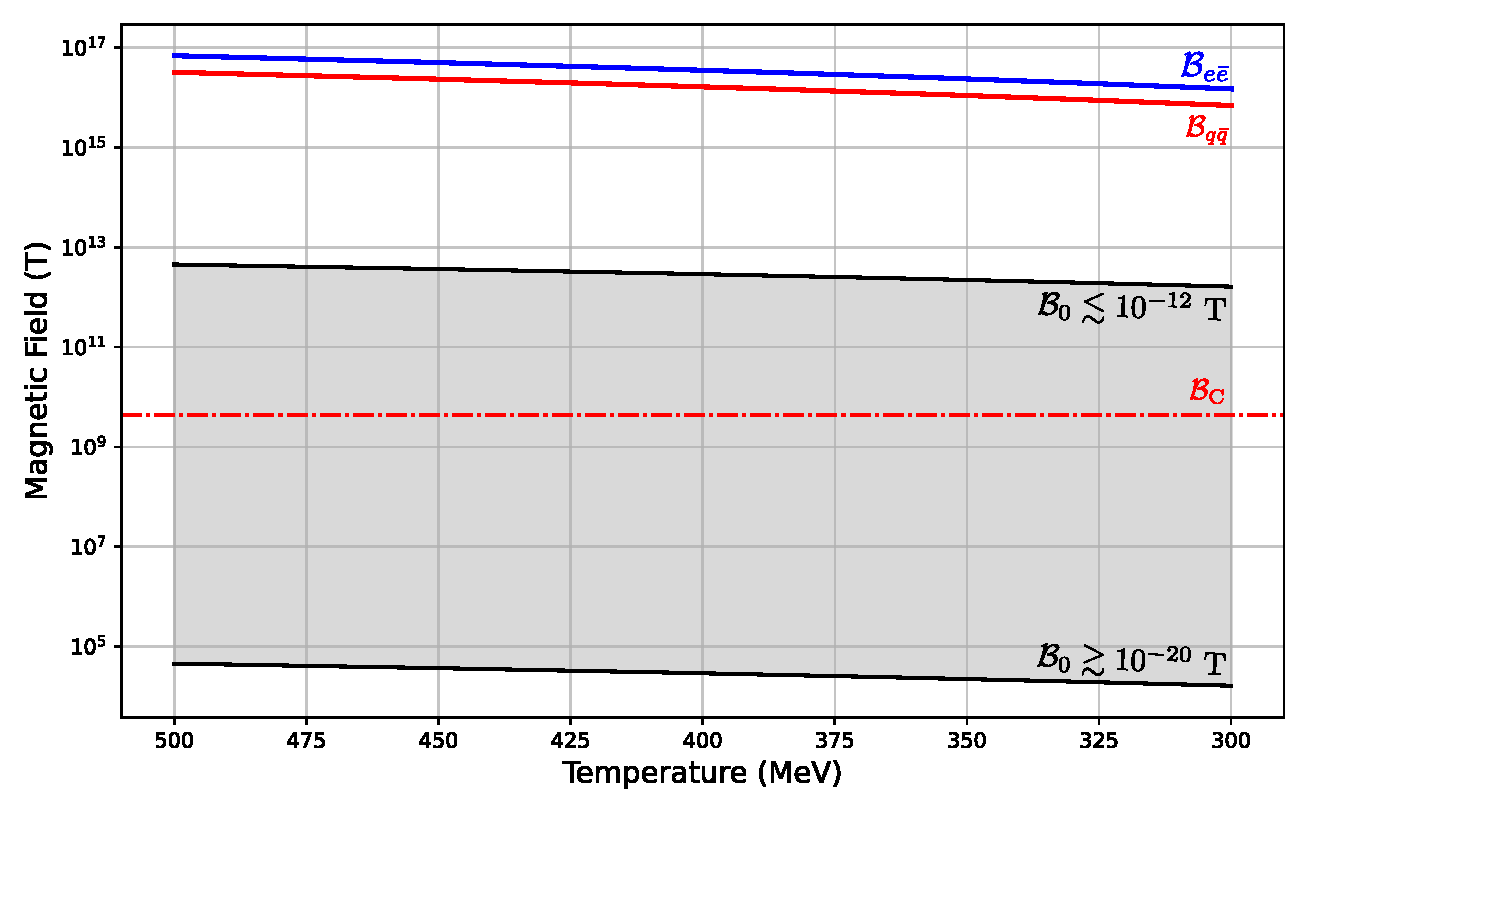
\includegraphics[width=0.90\columnwidth]{python/Figure_1.pdf}}
\caption{\label{Figure_1}Temperature dependence of several key magnetic field contributions in the early universe during the QGP epoch.}
\end{figure}

The black dash-dotted horizontal line in Fig.~\ref{Figure_1} marks the Schwinger critical field, \(\mathcal{B}_\mathrm{C}\approx4.41\times10^{9}~\mathrm{T}\). Superimposed are the maximum quark magnetization (red curve) and electron magnetization (blue curve) which are calculated below. The quark magnetization estimation ends well before hadronization which is marked by the red dashed vertical line at \(T_\mathrm{H}\approx150\MeV\). This is because near to the phase transformation at \(T_\mathrm{H}\), much less magnetically relevant heavy hadrons form.

We understand the primordial deconfined QGP phase of matter due to several decades of experimental effort; this new state of matter existed in the Universe for nearly \(25~\mathrm{\mu s}\) after the Big-Bang~\cite{Rafelski:2019twp,Rafelski:2023emw,Rafelski:2024fej}. However, there are differences between the QGP produced in the early Universe versus QGP produced in laboratory heavy-ion collisions. Of greatest importance is the presence of the lepton abundance in the early Universe. Laboratory formed QGP drops are too short-lived and too small to support a comparable high-density of leptons. The net baryon content of QGP-drops formed in laboratory experiments can also be vastly different from early Universe conditions where baryon-antibaryon asymmetry is nano-scale. A high QGP baryon content is found at relatively low energy heavy-ion collisions near to the presumed threshold for QGP formation~\cite{Letessier:2005qe}. In typically fixed target CERN experiments (NA61 today), baryon-rich conditions are explored and also expected to be present in astrophysical compact objects~\cite{Ghosh:2025sjn}. However, as the collision energy increases towards the highest available today, the incoming nuclear valance quarks escape from the QGP drop: CERN-LHC created QGP-drops as observed by ALICE and CMS experiments have relatively low net baryon density mirroring the prevailing conditions in the primordial Universe~\cite{Letessier:2005qe}. 

In this work we expand our prior spin magnetization study~\cite{Steinmetz:2023nsc,Steinmetz:2023ucp} to consider the role of light-quark magnetization in the primordial QGP Universe, focusing on the interplay between quarks, leptons, and magnetic fields. The presence of strong magnetic fields in the primordial QGP Universe could have significantly affected the equilibrium properties of Standard Model particles in the earliest moments after the Big-Bang~\cite{Durrer:2013pga,Subramanian:2015lua}. EM response of QGP is of considerable theoretical interest~\cite{Grayson:2022asf,Shovkovy:2022bnd,Ghosh:2024fkg} and such magnetic fields have long been thought to be connected to baryon asymmetry~\cite{Vachaspati:1991nm,Baym:1995fk}. Chiral magnetism in QGP has also been studied~\cite{Fukushima:2008xe,Boyarsky:2011uy,Bali:2011qj}.

We first argue that quark magnetism in cosmic QGP cannot be ignored. In Table~\ref{tab:particle_properties}, we list the relevant properties of select particles present in the QGP epoch of the Universe. The magnetic moment \(\mu\) is given in units of the Bohr magneton \(\mu_{B}\equiv e\hbar/2m_{e}\approx5.788\times10^{-11}\ \mathrm{MeV\;T}^{-1}\). The degrees of freedom (dof.) \(\mathfrak{g}=n_{S}\times n_{C}\) is the number of spin \(n_\mathrm{S}\) and color \(n_\mathrm{C}\) states available to the particle. We evaluate the magneton with gyromagnetic factor \(g=2\), while strong interaction corrections suggest a larger value for quarks. For each particle seen in Table~\ref{tab:particle_properties}, there is an antiparticle with opposite sign of magnetic moment. 
\begin{table}[h]
\centering
\caption{Properties of select particles}
\label{tab:particle_properties}
\begin{tabular}{@{}lllll@{}}
\toprule
\textbf{Particle} & \textbf{Mass} \([\approx\mathrm{MeV}]\) & \textbf{Charge} & \textbf{Magneton} \([\mu/\mu_{B}]\) & \(\mathfrak{g}\) \textbf{dof.} \\ 
\midrule
Electron \((e)\) & 0.511 & \(-1\) & \(-1\) & 2 \\
Muon \((\mu)\) & 105.7 & \(-1\) & \(-0.00484\) & 2 \\
Tau \((\mu)\) & 1776.9 & \(-1\) & \(-0.000288\) & 2 \\
\midrule
Up \((u)\) & 2.2 & \(+2/3\) & \(+0.155\) & 6 \\
Down \((d)\) & 4.7 & \(-1/3\) & \(-0.0362\) & 6 \\
Strange \((s)\) & 96 & \(-1/3\) & \(-0.00177\) & 6 \\
Charm \((c)\) & 1270 & \(+2/3\) & \(+0.000268\) & 6 \\ 
\bottomrule
\end{tabular}
\end{table}

The electron-positron and light-quark gases, especially up-quarks, are the magnetically most relevant particles in the QGP epoch due to their charge and low mass. The up-quark content is comparable to that of electrons since both are very relativistic particles considering \(k_{B}T=300\,\mathrm{MeV}\gg m_i c^{2}\). Their number densities \(n_{i}\) would then follow a massless fermion gas given by
\begin{align}
n_{i}(T) = \mathfrak{g}_{i}\frac{3}{4}\frac{\zeta(3)}{\pi^{2}}\left(\frac{k_{B}T}{\hbar c}\right)^{3}\,,
\end{align}
where \(\zeta(3)\approx1.202\) is the Riemann-Zeta function. The ratio of contribution to magnetism from light-quarks compared to leptons is thus solely rooted in their comparable magnetic moment and greater degeneracy. The estimated total cosmic magnetic flux strength is therefore derived from the sum of external flux density, and the medium polarization of the most magnetically active particles \((i)\) and antiparticles \((\bar{i})\), given by
\begin{align}
\mathcal{B}_\mathrm{total}=\mathcal{B}_\mathrm{ext.}+\mu_{0}\sum_{i} M_{i\bar{i}}\,,
\end{align}
where \(M=\mathcal{M}/V\) is the magnetic moment density, \(\mathcal{M}\) is the magnetization, and \(\mu_{0}\) is the vacuum permeability (not to be confused with magnetic moment). Therefore at \(k_{B}T=300~\mathrm{MeV}\) for up-quark and electrons, we obtain as an upper bound
\begin{align}
\label{eq:estimate}
\mu_{0}M_{u\bar{u}}\vert_{T=300\MeV} = \mu_{0}\mathcal{M}_{u\bar{u}}/V = \mu_{0}\mu_{u}(n_{u}+n_{\bar{u}}) \simeq 6.958\times10^{15}~\mathrm{T} \,,\qquad
M_{e\bar{e}}=M_{u\bar{u}}\frac{\mathfrak{g}_{e}}{\mathfrak{g}_{u}} \frac{\mu_{e}}{\mu_{u}} \simeq 2.15 M_{u\bar{u}}\,.
\end{align}
The estimate presented in \req{eq:estimate}, assumes that all strongly interacting quark magnetic moments align in a suitable manner with the electron generated magnetic field to amplify it further. This type of ferromagnetic alignment amplifies the lepton generated magnetization \(\sim 10^{6}\) times the critical magnetic field strength \(\mathcal{B}_\mathrm{C}\equiv m_{e}^{2}c^{2}/e\hbar\approx 4.41\times10^{9}\ \mathrm{T}\). This is comparable to the estimated maximum stellar core magnetic field strength within magnetars~\cite{Ferrer:2010wz} and \(\sim 10^5\) times stronger than their estimated surface field strength~\cite{Kaspi:2017fwg}.

This discussion suggests that even a weakly polarized (pico-scale) primordial lepton-quark Fermi gas would have a significant impact on the early Universe, as shown in Fig.~\ref{Figure_1}, with light-quarks contributing on par with leptons. While leptons remain dominant (within about a factor of 2), they are not the sole source of Fermi spin magnetization. We provide a theoretical outline and point to where future efforts may be directed in the sections below. For recent work on spin polarization modeled in relativistic hydrodynamics, see Refs.~\cite{Florkowski:2024cif,Bhadury:2024whs,Becattini:2024uha,Singh:2024cub}.

%%%%%%%%%%%%%%%%%%%%%%%%
\section{Magnetization of a polarized gas}
\label{sec:magnetization}
%%%%%%%%%%%%%%%%%%%%%%%%
We consider a free but magnetized fermion gas in the temperature range \(500\MeV>T\gtrsim150\MeV\) composed of light-quark species \(q \in {u,d}\) and electrons (and their antiparticles). As the magneton scales with \(\mu \propto 1/m\), these species are magnetically the most relevant due to their lighter masses (see Table~\ref{tab:particle_properties}) and consequently larger magnetic moments. For relativistic species under the conditions of thermal and chemical equilibrium~\cite{Elze:1980er}, as was the case in the primordial Universe, the chemical potential \(\eta\) of each particle is opposite in sign to that of its antiparticle
\begin{align}
\label{eq:equilibirum_conditions}
\eta_{q}=T\ln\lambda_{q}\,,\qquad
\lambda_{q}=1/\lambda_{\bar{q}}\,,\qquad
\eta_{q}=-\eta_{\bar{q}}\,,
\end{align}
where \(\lambda\) is the fugacity. The magnetic dipole of a particle is also opposite in sign to its antiparticle $\mu_{i}=-\mu_{\bar{i}}$ as charge is flipped. Any deviation from this condition would represent a violation of CPT~\cite{Colladay:1996iz,Bluhm:1997ci,BASE:2016yuo}. During this period, particle-antiparticle pairs of quark-antiquarks were freely produced and annihilated through photon- and gluon-mediated processes, represented by \(q+\bar{q}\rightleftharpoons2\gamma\) and \(q+\bar{q}\rightleftharpoons2g\). We note that the entropy conserving expansion of the Universe is extremely slow compared to the relevant collision reaction times during the QGP epoch~\cite{Yang:2024ret}.

Accounting for the internal energy $U$ of magnetized QGP, including the energies of neutrinos~\cite{Birrell:2014ona}, involves the following properties: 
\begin{itemize}
\item[(a)] The energy of adding or removing a baryon $\eta_{B}B$ where \(B\) is baryon number,
\item[(b)] the energy of adding or removing a lepton $\eta_{\ell}(N_{\ell}-N_{\ell})$ with $\ell\in {e,\nu}$, 
\item[(c)] the magnetic energy $\mathcal{M}\mathcal{B}$ where $\mathcal{M}$ is the net magnetization and $\mathcal{B}$ is the magnetic field strength and
\item[(d)] the electromagnetic energy density generated by the external magnetic field.
\end{itemize}

The dependency of $U$ on $\mathcal{M}$ reflects that $\mathcal{B}$ is the incremental energy cost to change the magnetization by flipping the spin of a particle~\cite{Bali:2014kia}. Therefore, this makes magnetization $\mathcal{M}$ an extensive property of the system which changes with particle number. We see this explicitly by writing the total spin magnetization as the sum over all particles $i\in{1,\ldots,k}$
\begin{align}
\label{eq:dipole}
\mathcal{M} = \sum_{i=1}^{k}(\mu_{i}N_{i}^{\uparrow} + \mu_{\bar{i}}N_{\bar{i}}^{\uparrow} - \mu_{i}N_{i}^{\downarrow} - \mu_{\bar{i}}N_{\bar{i}}^{\downarrow})\,,\qquad
N_{i} = N_{i}^{\uparrow} + N_{i}^{\downarrow}\,.
\end{align}
The $\uparrow\downarrow$ notation refers to spin-up $(\uparrow)$ and spin-down $(\downarrow)$ states along the direction of the external field. Therefore, $N_{i}^{\uparrow\downarrow}$ refers to the $i$-th constituent population number in either spin-up or spin-down orientation. The signs of each term in \req{eq:dipole} arises from the sign of the spin eigenvalue. While \req{eq:dipole} presumably includes contributions from each particle with a magnetic dipole, we expect the magnetization to be dominated by electron-positrons and the lightest quarks. Therefore we sum over $i\in{u,d,e}$
\begin{align}
\notag\mathcal{M} \approx &+|\mu_{u}|(N_{u}^{\uparrow}-N_{\bar{u}}^{\uparrow})-|\mu_{u}|(N_{u}^{\downarrow}-N_{\bar{u}}^{\downarrow})\\
\notag &-|\mu_{d}|(N_{d}^{\uparrow}-N_{\bar{d}}^{\uparrow})+|\mu_{d}|(N_{d}^{\downarrow}-N_{\bar{d}}^{\downarrow})\\
\label{eq:dipole2}
&-|\mu_{e}|(N_{e}^{\uparrow}-N_{\bar{e}}^{\uparrow})+|\mu_{e}|(N_{e}^{\downarrow}-N_{\bar{e}}^{\downarrow})\,.
\end{align}

We recognize that \req{eq:dipole2} contains terms representing asymmetry in the spin alignment though we can organize them in two different ways: (a) we group terms of the same spin alignment or (b) we group terms of matter and antimatter. The second approach allows the definition of spin-asymmetry in terms of conserved quantities characterizing spin angular momentum. We define net spin-asymmetry numbers $\delta_{i}^{\uparrow\downarrow}$ and write
\begin{align}
\delta_{i}^{\uparrow\downarrow} &\equiv N_{i}^{\uparrow\downarrow}-N_{\bar{i}}^{\uparrow\downarrow}\,,\\
\mathcal{M} &= 
+|\mu_{u}|(\delta_{u}^{\uparrow}-\delta_{u}^{\downarrow})
-|\mu_{d}|(\delta_{d}^{\uparrow}-\delta_{d}^{\downarrow})
-|\mu_{e}|(\delta_{e}^{\uparrow}-\delta_{e}^{\downarrow})\,.
\end{align}
The net spin-asymmetry is the asymmetry of particles and antiparticles of the same spin. Therefore $\delta_{u}^{\uparrow}\neq0$ represents a situation where there are more up quarks than up antiquarks in the spin-up $\uparrow$ state.

%%%%%%%%%%%%%%%%%%%%%%%%
\section{Magnetized grand partition function}
\label{sec:partition}
%%%%%%%%%%%%%%%%%%%%%%%%
The partition function allows us to calculate various thermodynamic quantities by taking appropriate derivatives of the grand potential $\mathcal{F}$. In the temperature range considered $(500\MeV>T\gtrsim150\MeV)$, the lightest quarks act as essentially massless particles. Strange quarks can also be included albeit with mass corrections. It is worth remarking on the uniqueness of the situation: As magnetic moment scales inverse with mass, it is the particles which are most massless in character which contribute most to magnetization. The following section is written in natural units of \(\hbar=c=k_{B}=1\).

The relevant contributions to the magnetized primordial plasma arise from the quarks, gluons, leptons, and the vacuum. The grand potential in terms of the grand partition function $\mathcal{Z}$ is
\begin{align}
\label{eq:parts}
\mathcal{F} &= -T\ln\mathcal{Z}\,,\\
\ln\mathcal{Z}_{\mathrm{total}} &=
\ln\mathcal{Z}_{\mathrm{quarks}} +
\ln\mathcal{Z}_{\mathrm{gluons}} +
\ln\mathcal{Z}_{\mathrm{leptons}}+
\ln\mathcal{Z}_{\mathrm{vac.}}+\ldots 
\end{align}

We consider a homogeneous magnetic field domain defined along the $z$-axis with magnetic field magnitude $\mathcal{B}$. The volume $V=L^{3}$ is not necessarily infinite and defines the size of the homogeneous domain such that $\partial\mathcal{B}_{i}/\partial x_{j}\approx0$ for \(i,j \in {1,2,3}\). For a fermion species of charge $Q$, mass $m$, and g-factor $g$, the energy eigenvalues of the magnetized particles is given by~\cite{Steinmetz:2018ryf}
\begin{align}
\label{eq:energystates}
E(p_{z},n,s)=\sqrt{m^{2}+p_{z}^{2}+2|Q|\mathcal{B}\left(n+\frac{1}{2}-\frac{g}{2}s\right)}\,,
\end{align}
where $E$ are the relativistic Landau energy eigenvalues. The micro-state energies depend on longitudinal momentum \(p_{z}\), spin $s\in\pm1/2$, and Landau orbital $n\in0,1,2,3,\ldots$ quantum numbers. It is helpful to introduce a spin-dependent auxiliary mass $m(s)$ via
\begin{align}
\label{eq:spinmass}
m^{2}(s) &\equiv m^{2} - |Q|\mathcal{B}\,g s\,.
\end{align}

The power and utility of the partition function in statistical systems is found by examining the Fermi integral in various limits and expansions. We state the Fermi-Dirac distribution given by
\begin{align}
F\left(E - \sigma\eta\right) = \frac{1}{e^{(E - \sigma\eta)/T} + 1}\,.
\end{align}
The parameter \(\sigma \in {\pm1}\) describes both matter and antimatter states satisfying \req{eq:equilibirum_conditions}. We can evaluate \req{eq:parts} by utilizing Euler-Maclaurin integration over the Landau levels \(n\) (see details in Ref.~\cite{Steinmetz:2023nsc}) and write the partition function in spherical coordinates \(d\mathbf{p}^{3}=4\pi p^{2}dp\). We substitute coordinates and integrate by parts yielding
\begin{align}
\label{eq:partition_byparts}
\ln\mathcal{Z} &= \frac{2 n_\mathrm{C}V}{(2\pi)^{2}} \sum_{s}^{\pm1/2}\sum_{\sigma}^{\pm1}\int_{0}^{\infty} \frac{dp}{3T} \, \frac{p^4}{E}F\left(E - \sigma\eta\right)\,.
\end{align}
The form of the partition function expressed by \req{eq:partition_byparts} more directly lets us evaluate thermodynamic quantities in terms of Fermi integrals~\cite{Elze:1980er,Birrell:2024bdb}. \req{eq:partition_byparts} also sums over spin \(s\) and matter-antimatter \(\sigma\) states. However, integrating over momentum is not an ideal description as relativistic expansions in momentum yield series that are only semi-convergent. 

%%%%%%%%%%%%%%%%%%%%%%%%
\subsection{Dimensionless change of variables}
\label{sec:dimensionless}
%%%%%%%%%%%%%%%%%%%%%%%%
To simplify the integration process, we introduce dimensionless variables by normalizing relevant physical quantities with the temperature \( T \). This approach renders the equations dimensionless and highlights the thermal contributions explicitly. The dimensionless variables are defined as
\begin{align}
\label{eq:dimensionless_variables}
p_{T} = \frac{p}{T}, \qquad E_{T}(p_{T},s) = \frac{E(p,s)}{T}, \qquad \eta_{T} = \frac{\eta}{T}\,, \qquad m_{T}(s) = \frac{m(s)}{T}\,.
\end{align}
This yields momentum-like \(p_{T}\), energy-like \(E_{T}\), chemical potential-like \(\eta_{T}\) and mass-like \(m_{T}\) parameters. Using the relativistic dispersion relation, the dimensionless energy \( E_{T} \) can be expressed in terms of \( p_{T} \) and \( m_{T} \)
\begin{align}
E_{T} = \frac{E}{T} = \sqrt{p_{T}^{2} + m_{T}^{2}}\,.
\end{align}
The differential \( dp_{T} \) and \( dE_{T} \) transform as
\begin{align}
dp = T \, dp_{T}\,,\qquad p_{T}dp_{T} = E_{T} dE_{T}\,,
\end{align}
and the limits of integration change accordingly
\begin{equation}
p_{T} = 0 \quad \Rightarrow \quad E_{T} = m_{T}, \quad p_{T} \to \infty \quad \Rightarrow \quad E_{T} \to \infty.
\end{equation}
Substituting these dimensionless variables and differentials into the partition function \( \ln\mathcal{Z} \), we obtain expressions for both momentum-like \(p_{T}\) integration and energy-like \(E_{T}\) integration
\begin{align}
\label{eq:dimensionless_partition}
\ln\mathcal{Z} 
&= \frac{2 n_\mathrm{C} V}{(2\pi)^{2}} \frac{T^{3}}{3} \sum_{s}^{\pm1/2}\sum_{\sigma}^{\pm1} \int_{0}^{\infty} dp_{T} \, \frac{p_{T}^{4}}{\sqrt{p_{T}^{2} + m_{T}^{2}}} \, F\left(\sqrt{p_{T}^{2} + m_{T}^{2}} - \sigma\eta_{T}\right)\,,\\
\label{eq:dimensionless_partition2}
&= \frac{2 n_\mathrm{C} V}{(2\pi)^{2}} \frac{T^{3}}{3} \sum_{s}^{\pm1/2}\sum_{\sigma}^{\pm1} \int_{m_{T}}^{\infty} dE_{T} \, (E_{T}^2-m_{T}^2)^{3/2} F\left(E_{T} - \sigma\eta_{T}\right)\,.
\end{align}
In this formulation, it is evident that the logarithm of the partition function scales as \( \ln\mathcal{Z} \propto T^{3} \), consistent with the expected thermodynamic behavior for a relativistic gas in three spatial dimensions.

%%%%%%%%%%%%%%%%%%%%%%%%
\subsection{Evaluation of magnetization from the dimensionless partition function}
\label{sec:magnetization_evaluation}
%%%%%%%%%%%%%%%%%%%%%%%%
Given the dimensionless form of the partition function \req{eq:dimensionless_partition}, we proceed to evaluate the magnetization. We emphasize that the dimensionless mass \(m_{T}(\mathcal{B},s)\) depends on the magnetic field and spin via \req{eq:spinmass}. Taking the derivative of the free energy \(\mathcal{F} = -T \ln\mathcal{Z}\) with respect to the magnetic field \(\mathcal{B}\), we obtain the magnetization
\begin{align}
\label{eq:magnetization_def}
\mathcal{M} = \left( \frac{\partial \mathcal{F}}{\partial \mathcal{B}} \right) = -T \left( \frac{\partial \ln\mathcal{Z}}{\partial \mathcal{B}} \right)\,.
\end{align} 
Since \(\ln\mathcal{Z}\) depends on \(\mathcal{B}\) solely through \(m_{T}\), we apply the chain rule
\begin{align}
\label{eq:chain_rule}
\frac{\partial \ln\mathcal{Z}}{\partial \mathcal{B}} = \frac{\partial \ln\mathcal{Z}}{\partial m_{T}} \frac{\partial m_{T}}{\partial \mathcal{B}}\,,\qquad
\frac{\partial m_{T}}{\partial \mathcal{B}} = -\frac{g|Q|s}{2m_{T}T^2}\,.
\end{align}
Taking the derivative of the partition function \req{eq:dimensionless_partition} with respect to \(m_{T}\), we write
\begin{equation}
\frac{\partial \ln \mathcal{Z}}{\partial m_{T}} = \frac{2 n_\mathrm{C} V T^{3}}{3 (2\pi)^{2}} \sum_{s}^{\pm1/2}\sum_{\sigma}^{\pm1} \int_{0}^{\infty} dp_{T} \, \frac{\partial}{\partial m_{T}} \left( \frac{p_{T}^{4}}{\sqrt{p_{T}^{2} + m_{T}^{2}}} F\left(\sqrt{p_{T}^{2} + m_{T}^{2}} - \sigma \eta_{T} \right) \right).
\end{equation}
Given that \(E_{T} = \sqrt{p_{T}^{2} + m_{T}^{2}}\), then \(\partial E_{T} / \partial m_{T} = m_{T} / E_{T}\). The derivative of the integrand is therefore
\begin{equation}
\frac{\partial}{\partial m_{T}} \left( \frac{p_{T}^{4}}{E_{T}} F(E_{T} - \sigma\eta_{T}) \right) = \frac{p_{T}^{4}}{E_{T}} \frac{\partial F}{\partial E_{T}} \frac{\partial E_{T}}{\partial m_{T}} + F(E_{T} - \sigma\eta_{T}) \frac{\partial}{\partial m_{T}} \left( \frac{p_{T}^{4}}{E_{T}} \right).
\end{equation}
Hereafter we write \(F'=\partial F/\partial E_{T}\). The second term evaluates to
\begin{equation}
\frac{\partial}{\partial m_{T}} \left( \frac{p_{T}^{4}}{E_{T}} \right) = -\frac{p_{T}^{4} m_{T}}{E_{T}^{3}}.
\end{equation}
Substituting these results back, the integrand becomes
\begin{equation}
\frac{\partial}{\partial m_{T}} \left( \frac{p_{T}^{4}}{E_{T}} F(E_{T} - \sigma\eta_{T}) \right) = \frac{p_{T}^{4} m_{T}}{E_{T}^{2}} F'(E_{T} - \sigma\eta_{T}) - \frac{p_{T}^{4} m_{T}}{E_{T}^{3}} F(E_{T} - \sigma\eta_{T}).
\end{equation}
Replacing \(E_{T}\) with \(\sqrt{p_{T}^{2} + m_{T}^{2}}\), the derivative of \(\ln \mathcal{Z}\) is
\begin{align}
\frac{\partial \ln \mathcal{Z}}{\partial m_{T}} &= \frac{2 n_\mathrm{C} V T^{3}}{3 (2\pi)^{2}} \sum_{s}^{\pm1/2}\sum_{\sigma}^{\pm1} \int_{0}^{\infty} dp_{T} \, p_{T}^{4} m_{T}
\left( \frac{F'\left( \sqrt{p_{T}^{2} + m_{T}^{2}} - \sigma\eta_{T} \right)}{p_{T}^{2} + m_{T}^{2}} - \frac{F\left( \sqrt{p_{T}^{2} + m_{T}^{2}} - \sigma\eta_{T} \right)}{(p_{T}^{2} + m_{T}^{2})^{3/2}} \right).
\end{align}
This result provides the explicit form of \(\partial \ln \mathcal{Z}/\partial m_{T}\) in terms of \(F\) and its derivative \(F'\), with all dependencies on \(m_{T}\) and \(p_{T}\) made explicit.

Given that \( F(x) = 1/(e^{x} + 1) \) is the Fermi-Dirac distribution, its derivative is
\begin{equation}
F'(x) = \frac{dF}{dx} = -\frac{e^{x}}{(e^{x} + 1)^2} = -F(x)\left[1 - F(x)\right].
\end{equation}
We replace \( F'(x) \) in the expression for the derivative of the integrand yielding
\begin{align}
\notag
&\int_{0}^{\infty} dp_{T} \, p_{T}^{4} m_{T} \left( -\frac{F(E_{T} - \sigma\eta_{T})\left[1 - F(E_{T} - \sigma\eta_{T})\right]}{E_{T}^{2}} - \frac{F(E_{T} - \sigma\eta_{T})}{E_{T}^{3}} \right) =\\*
&\int_{m_{T}}^{\infty} dE_{T} \, \left(E_{T}^{2} - m_{T}^{2}\right)^{3/2} m_{T} \left( -\frac{F(E_{T} - \sigma\eta_{T})\left[1 - F(E_{T} - \sigma\eta_{T})\right]}{E_{T}} - \frac{F(E_{T} - \sigma\eta_{T})}{E_{T}^{2}} \right).
\end{align}
Substituting the expression for \(\partial \ln \mathcal{Z}/\partial m_{T}\) into \req{eq:magnetization_def} and \req{eq:chain_rule}, we obtain the magnetization
\begin{align}
\notag
\mathcal{M} &= -\frac{g|Q|}{2 T}\cdot\frac{2 n_\mathrm{C} V T^{3}}{3 (2\pi)^{2}} \sum_{s}^{\pm1/2} s \sum_{\sigma}^{\pm1} \int_{m_{T}(s)}^{\infty} dE_{T} \, \left(E_{T}^{2} - m_{T}^{2}(s)\right)^{3/2} \\
\label{eq:mag_form}
&\times
\left[ \frac{F(E_{T} - \sigma\eta_{T})\left(1 - F(E_{T} - \sigma\eta_{T})\right)}{E_{T}} + \frac{F(E_{T} - \sigma\eta_{T})}{E_{T}^{2}} \right].
\end{align}
In much how we expected the free energy to be \(\ln\mathcal{Z}\sim T^{3}\), we see the magnetization is \(\mathcal{M}\sim T^{2}\) in natural units via dimensional analysis. This is in agreement to our prior work~\cite{Steinmetz:2023nsc,Steinmetz:2023ucp} where we evaluated the magnetization in the Boltzmann limit~\cite{Steinmetz:2023nsc} with \(T\ll m_e\). The benefit of expressing the magnetization in the form of \req{eq:mag_form} is that the integrand within the brackets \([\ldots]\) entirely contains the Fermi-Dirac distribution scaled by energy without mass (or magnetic fields) except as a boundary condition on the integration. This makes it suitable for numerical evaluation and comparison to the Boltzmann limit which will be the subject of future efforts.

%%%%%%%%%%%%%%%%%%%%%%%%
\section{Conclusions}
\label{sec:conclusions}
%%%%%%%%%%%%%%%%%%%%%%%%
Our estimates indicate that a modest (pico-scale) degree of spin polarization in the light-quark and electron-positron sectors could lead to cosmic primordial magnetic fields of enormous magnitude consistent with intergalactic fields observed today. This suggests that strong polarization domains can randomly aid to create relevant large scale structure. Such a ferromagnetic-like response, if facilitated by the strong coupling among quarks, could generate fields on the order of \(10^{16}\) Tesla during the QGP epoch. These values exceed both the critical Schwinger field and the characteristic surface fields of magnetars by several orders of magnitude and are comparable to estimates of magnetar stellar cores. Such fields remain in the bounds found at this high temperature by extrapolating back in time the large scale magnetic fields of the present day (see Fig.~\ref{Figure_1}).

In this work we have proposed a theoretical framework for evaluating the spin magnetization of QGP under conditions akin to those of the primordial Universe. By employing a grand partition function formalism (see \req{eq:parts}) and rigorously evaluating magnetized Fermi-Dirac integrals, both in their standard and dimensionless forms (\req{eq:dimensionless_partition} and \req{eq:dimensionless_partition2}), we derived explicit expressions that capture the dependence of the magnetization on temperature, particle masses, and magnetic field strength. Notably, our analysis shows that the magnetization scales as \(T^2\) (see \req{eq:mag_form}), in agreement with the expected thermodynamic behavior of a magnetized relativistic gas in three spatial dimensions.

While the present treatment considers an idealized free fermion gas, with the magnetization defined in \req{eq:dipole}, it provides a starting point for future investigations to incorporate additional physical effects such as QCD interactions, finite volume corrections, and non-equilibrium dynamics. Moreover, exploring the interplay between spin magnetization and other dynamic cosmological processes relevant to the evolution of large-scale magnetic fields remains an important avenue for further research.\\

%%%%%%%%%%%%%%%%%%%%%%%%%%%%%%%%%%%%%%%%%%%%
\textbf{Acknowledgment:} 
One of us (JR) thanks Tamas Bir\'o and the Wigner Hun-Ren Research Center for their kind hospitality in Budapest during the PP2024 conference, supported by NKFIH (Hungarian National Office for Research, Development and Innovation) under awards 2022-2.1.1-NL-2022-00002 and 2020-2.1.1-ED-2024-00314. This meeting and the related research report motivate the presentation of these recently obtained results. The authors and this work were not supported by any sponsor.

%%%%%%%%%%%%%%%%%%%%%%%%%
%%%%%%%%%%%%%%%%%%%%%%%%
\bibliographystyle{sn-aps}
\bibliography{short-note-qcd.bib}
%%%%%%%%%%%%%%%%%%%%%%%%
\end{document}
